
\ifdefined\FIGINPUT\else
  \documentclass[border=4pt]{standalone}
  \usepackage{tikz}
  \usepackage{amsmath}
  \usetikzlibrary{arrows.meta,positioning,fit,backgrounds,calc}
  \begin{document}
\fi

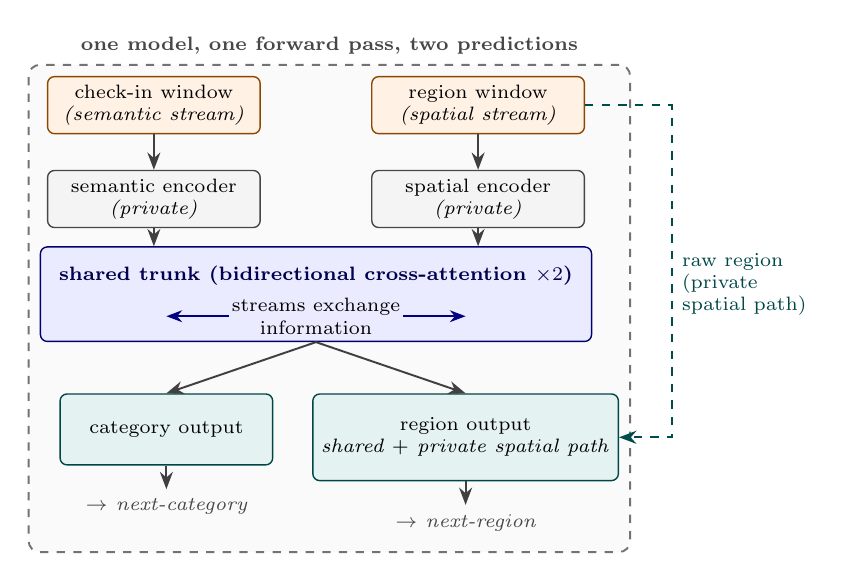
\begin{tikzpicture}[
    >={Stealth[length=2.2mm]},
    font=\footnotesize,
    box/.style={draw, rounded corners=2.5pt, align=center, inner sep=3pt,
                minimum height=7mm, line width=0.5pt, font=\scriptsize},
    inblk/.style={box, fill=orange!10, draw=orange!55!black, minimum width=27mm,
                  font=\scriptsize},
    enc/.style={box, fill=gray!9, draw=gray!55!black, minimum width=27mm},
    shared/.style={box, fill=blue!8, draw=blue!45!black, minimum width=70mm,
                   minimum height=12mm},
    cathead/.style={box, fill=teal!10, draw=teal!55!black, minimum width=27mm,
                    minimum height=9mm},
    reghead/.style={box, fill=teal!10, draw=teal!55!black, minimum width=33mm,
                    minimum height=11mm},
    outlbl/.style={font=\scriptsize\itshape, text=black!72},
    flow/.style={->, line width=0.7pt, draw=black!75},
    kv/.style={{Stealth[length=2mm]}-{Stealth[length=2mm]}, line width=0.9pt,
               draw=blue!50!black},
    skip/.style={->, line width=0.8pt, draw=teal!60!black, dashed},
  ]

  \node[inblk] (inc) {check-in window\\\textit{(semantic stream)}};
  \node[inblk, right=14mm of inc] (inr) {region window\\\textit{(spatial stream)}};

  \node[enc, below=4.5mm of inc] (enca) {semantic encoder\\\scriptsize\textit{(private)}};
  \node[enc, below=4.5mm of inr] (encb) {spatial encoder\\\scriptsize\textit{(private)}};

  \node[shared, below=6mm of $(enca)!0.5!(encb)$] (cross) {};
  \node[anchor=north, font=\scriptsize\bfseries, text=blue!30!black]
       at ([yshift=-1.3mm]cross.north) {shared trunk (bidirectional cross-attention $\times 2$)};

  \node[cathead, below=6.5mm of cross.south, anchor=north, xshift=-19mm] (cath)
       {category output};
  \node[reghead, below=6.5mm of cross.south, anchor=north, xshift=19mm] (regh)
       {region output\\\scriptsize\textit{shared $+$ private spatial path}};

  \node[outlbl, below=3mm of cath] (oc) {$\rightarrow$ next-category};
  \node[outlbl, below=3mm of regh] (orr) {$\rightarrow$ next-region};

  \draw[flow] (inc) -- (enca);
  \draw[flow] (inr) -- (encb);
  \draw[flow] (enca.south) -- (enca.south |- cross.north);
  \draw[flow] (encb.south) -- (encb.south |- cross.north);
  \draw[kv] ([xshift=-19mm,yshift=-2.8mm]cross.center) -- ([xshift=19mm,yshift=-2.8mm]cross.center)
       node[pos=0.5, fill=blue!8, inner sep=1pt, font=\scriptsize, align=center]
       {streams exchange\\information};
  \draw[flow] (cross.south) -- (cath.north);
  \draw[flow] (cross.south) -- (regh.north);
  \draw[flow] (cath.south) -- (oc.north);
  \draw[flow] (regh.south) -- (orr.north);
  \draw[skip] (inr.east) -- ++(11mm,0) |- (regh.east)
       node[pos=0.27, right, font=\scriptsize, text=teal!55!black, align=left]
       {raw region\\(private\\spatial path)};

  \begin{scope}[on background layer]
    \node[draw, dashed, rounded corners=4pt, line width=0.7pt, draw=black!55,
          fill=black!2, inner sep=4pt,
          fit=(inc)(inr)(enca)(encb)(cross)(cath)(regh)(oc)(orr)] (model) {};
  \end{scope}
  \node[anchor=south, font=\scriptsize\bfseries, text=black!72]
        at (model.north) {one model, one forward pass, two predictions};

\end{tikzpicture}

\ifdefined\FIGINPUT\else
  \end{document}
\fi
